\section{Thuật toán Not So Naïve}
\subsection{Đặc điểm chính}
Thuật toán Not So Naive là một cải tiến đơn giản so với thuật toán Naive
trong bài toán tìm kiếm xâu. Thay vì so sánh lại toàn bộ mẫu tại mỗi vị
trí, thuật toán sử dụng một nhận xét nhỏ về cấu trúc của mẫu để bỏ qua
một số vị trí không cần thiết, giúp giảm số phép so sánh trong thực tế.

Thuật toán có các đặc điểm sau:

\begin{itemize}
  \item Pha tiền xử lý thực hiện trong thời gian và không gian hằng số $O(1)$.
  \item Pha tìm kiếm có độ phức tạp thời gian $O(nm)$ trong trường hợp xấu nhất.
  \item Hiệu quả hơn thuật toán Naive theo hệ số trong trường hợp trung bình,
        tức là có tính chất \textit{sub-linear} nhẹ theo hệ số.
\end{itemize}

\subsection{Mô tả thuật toán}

Trong pha tìm kiếm của thuật toán Not So Naive, các phép so sánh ký tự
được thực hiện theo thứ tự vị trí của mẫu như sau:
$1, 2, \ldots, m-2, m-1, 0$.

Với mỗi lần thử, khi cửa sổ được đặt tại đoạn văn bản $y[j \mathinner{..} j+m-1]$:
\begin{itemize}
  \item Nếu $x[0] = x[1]$ và $x[1] \neq y[j+1]$, hoặc nếu $x[0] \neq x[1]$
        và $x[1] = y[j+1]$, thì mẫu được dịch sang phải $2$ vị trí sau lần
        thử đó.
  \item Trong các trường hợp còn lại, mẫu được dịch sang phải $1$ vị trí.
\end{itemize}

Nhờ vậy, pha tiền xử lý có thể thực hiện trong thời gian và không gian
hằng số $O(1)$. Pha tìm kiếm của thuật toán Not So Naive có độ phức tạp
thời gian bậc hai $O(nm)$ trong trường hợp xấu nhất, nhưng có tính chất
\textit{sub-linear} nhẹ theo hệ số trong trường hợp trung bình.

\subsection{Cài đặt bằng C++}
\begin{verbatim}
#include <string>
#include <vector>
#include <cstring>

std::vector<int> NSN(const std::string& x, const std::string& y) {
    int m = static_cast<int>(x.size());
    int n = static_cast<int>(y.size());
    std::vector<int> results;

    /* Preprocessing */
    int k, ell;
    if (x[0] == x[1]) {
        k   = 2;
        ell = 1;
    } else {
        k   = 1;
        ell = 2;
    }

    /* Searching */
    int j = 0;
    while (j <= n - m) {
        if (x[1] != y[j + 1]) {
            j += k;
        } else {
            if (std::memcmp(x.c_str() + 2, y.c_str() + j + 2, m - 2) == 0
                && x[0] == y[j])
                results.push_back(j); // OUTPUT(j)
            j += ell;
        }
    }

    return results;
}
\end{verbatim}

\subsection{Kiểm nghiệm thuật toán}
Với $k = 1$ và $\ell = 2$

Lần 1:
\begin{figure}[H]
    \centering
    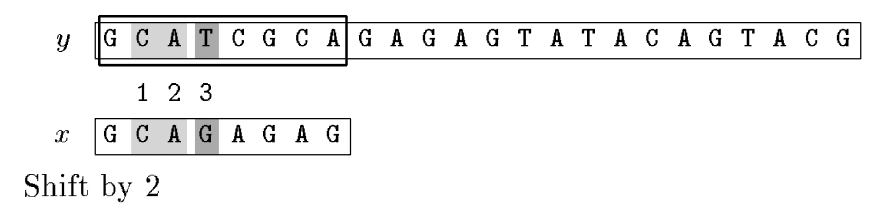
\includegraphics[width=10cm]{Images/2026-05-15-10-56-52.png}
    \caption{Bước 1 trong quá trình thực hiện thuật toán Not So Naive}
    \label{fig:not-so-naive-step-1}
\end{figure}

Lần 2:
\begin{figure}[H]
    \centering
    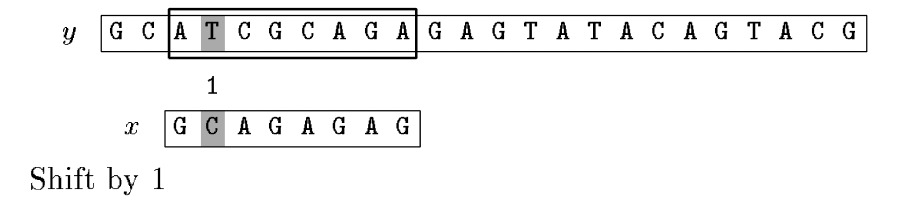
\includegraphics[width=10cm]{Images/2026-05-15-10-57-08.png}
    \caption{Bước 2 trong quá trình thực hiện thuật toán Not So Naive}
    \label{fig:not-so-naive-step-2}
\end{figure}

Lần 3:
\begin{figure}[H]
    \centering
    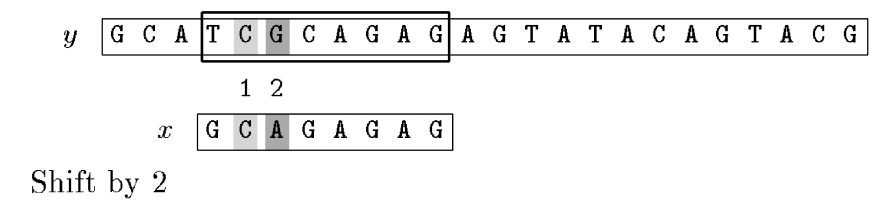
\includegraphics[width=10cm]{Images/2026-05-15-10-57-27.png}
    \caption{Bước 3 trong quá trình thực hiện thuật toán Not So Naive}
    \label{fig:not-so-naive-step-3}
\end{figure}

Lần 4:
\begin{figure}[H]
    \centering
    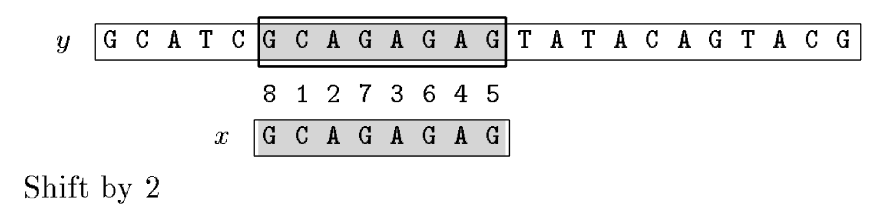
\includegraphics[width=10cm]{Images/2026-05-15-10-57-42.png}
    \caption{Bước 4 trong quá trình thực hiện thuật toán Not So Naive}
    \label{fig:not-so-naive-step-4}
\end{figure}

Lần 5:
\begin{figure}[H]
    \centering
    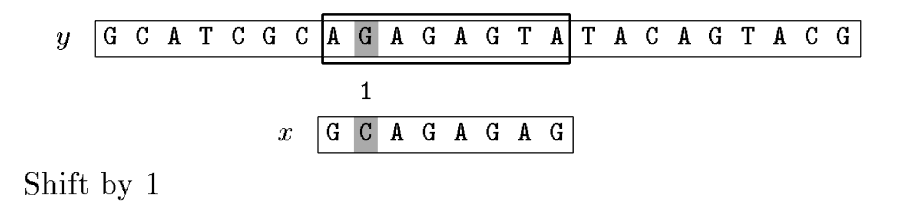
\includegraphics[width=10cm]{Images/2026-05-15-10-58-03.png}
    \caption{Bước 5 trong quá trình thực hiện thuật toán Not So Naive}
    \label{fig:not-so-naive-step-5}
\end{figure}

Lần 6:
\begin{figure}[H]
    \centering
    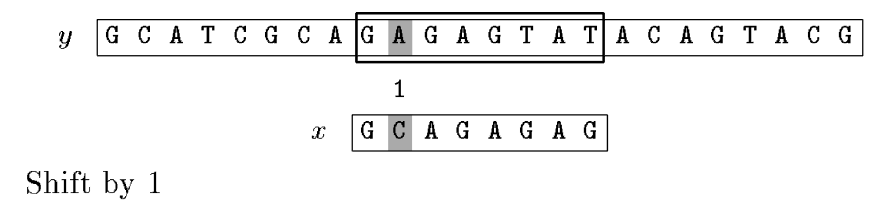
\includegraphics[width=10cm]{Images/2026-05-15-10-58-16.png}
    \caption{Bước 6 trong quá trình thực hiện thuật toán Not So Naive}
    \label{fig:not-so-naive-step-6}
\end{figure}

Lần 7:
\begin{figure}[H]
    \centering
    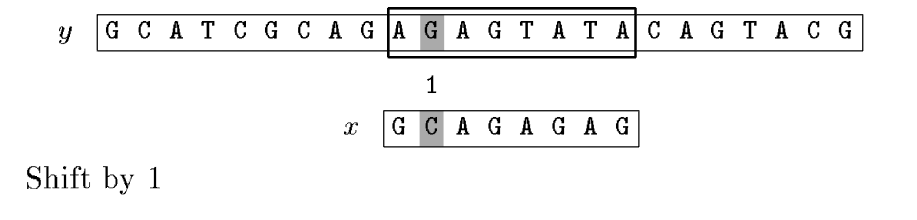
\includegraphics[width=10cm]{Images/2026-05-15-10-58-27.png}
    \caption{Bước 7 trong quá trình thực hiện thuật toán Not So Naive}
    \label{fig:not-so-naive-step-7}
\end{figure}

Lần 8:
\begin{figure}[H]
    \centering
    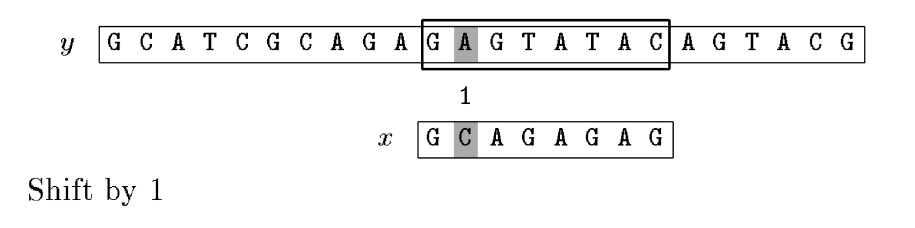
\includegraphics[width=10cm]{Images/2026-05-15-10-58-38.png}
    \caption{Bước 8 trong quá trình thực hiện thuật toán Not So Naive}
    \label{fig:not-so-naive-step-8}
\end{figure}

Lần 9:
\begin{figure}[H]
    \centering
    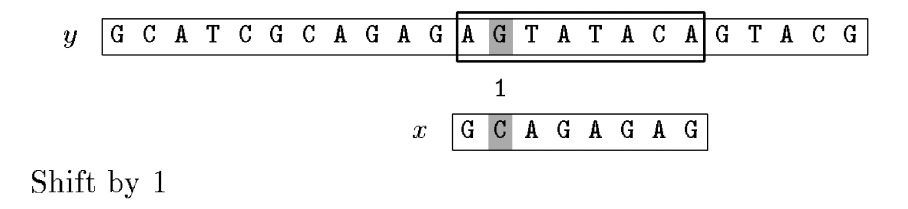
\includegraphics[width=10cm]{Images/2026-05-15-10-58-51.png}
    \caption{Bước 9 trong quá trình thực hiện thuật toán Not So Naive}
    \label{fig:not-so-naive-step-9}
\end{figure}

Lần 10:
\begin{figure}[H]
    \centering
    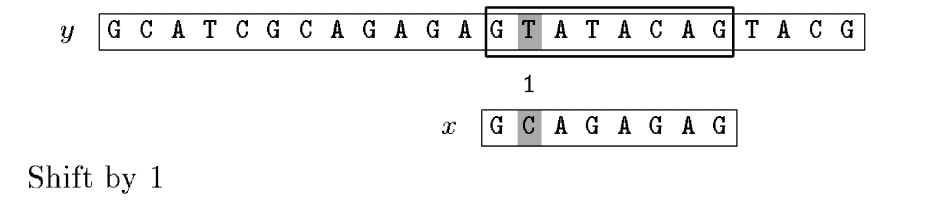
\includegraphics[width=10cm]{Images/2026-05-15-10-59-03.png}
    \caption{Bước 10 trong quá trình thực hiện thuật toán Not So Naive}
    \label{fig:not-so-naive-step-10}
\end{figure}

Lần 11:
\begin{figure}[H]
    \centering
    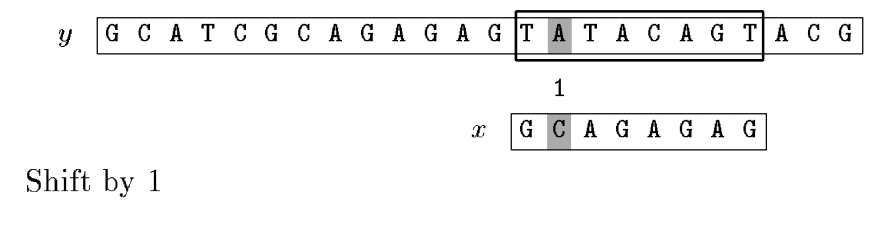
\includegraphics[width=10cm]{Images/2026-05-15-10-59-25.png}
    \caption{Bước 11 trong quá trình thực hiện thuật toán Not So Naive}
    \label{fig:not-so-naive-step-11}
\end{figure}

Lần 12:
\begin{figure}[H]
    \centering
    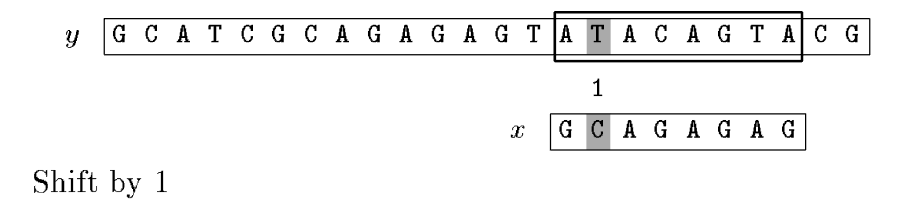
\includegraphics[width=10cm]{Images/2026-05-15-10-59-37.png}
    \caption{Bước 12 trong quá trình thực hiện thuật toán Not So Naive}
    \label{fig:not-so-naive-step-12}
\end{figure}

Lần 13:
\begin{figure}[H]
    \centering
    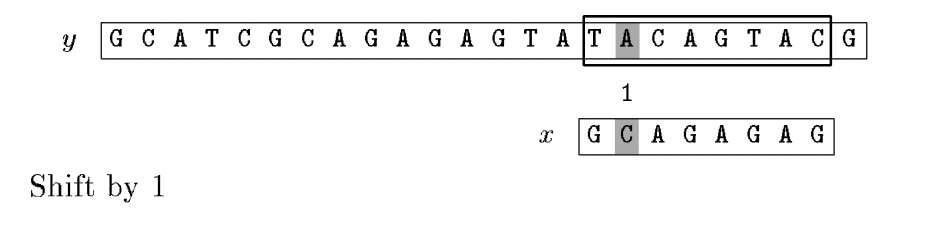
\includegraphics[width=10cm]{Images/2026-05-15-10-59-48.png}
    \caption{Bước 13 trong quá trình thực hiện thuật toán Not So Naive}
    \label{fig:not-so-naive-step-13}
\end{figure}

Lần 14:
\begin{figure}[H]
    \centering
    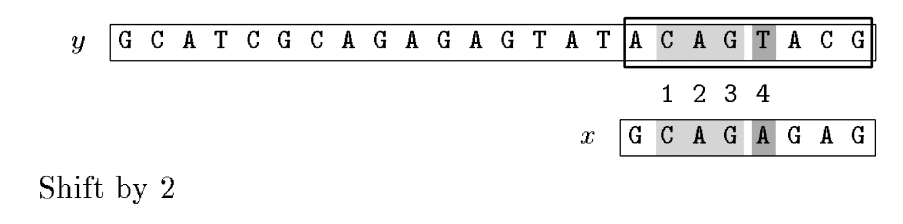
\includegraphics[width=10cm]{Images/2026-05-15-10-59-57.png}
    \caption{Bước 14 trong quá trình thực hiện thuật toán Not So Naive}
    \label{fig:not-so-naive-step-14}
\end{figure}

Thuật toán Not So Naive thực hiện 27 lần so khớp chuỗi trong ví dụ trên.